\documentclass[runningheads,a4paper]{llncs}

\usepackage{amssymb}
\setcounter{tocdepth}{3}
\usepackage{graphicx}
\usepackage{pgfplots}
\usepackage{float}
\usepackage{tabularx}
\usepgfplotslibrary{groupplots}

\usepackage{url}
\newcommand{\keywords}[1]{\par\addvspace\baselineskip
\noindent\keywordname\enspace\ignorespaces#1}

\begin{document}

\setlength{\tabcolsep}{12pt}

\mainmatter

\title{Fast Nearest Neighbour Classification}
\subtitle{\textnormal{\small{Seminar\\
Intelligent Software Systems\\
Summer semester 2015\\\vspace{1\baselineskip}
Lecturer: Stefan Fricke\\\vspace{2\baselineskip}
June 2016\\
Supervisor: Stephan Spiegel\\\vspace{1\baselineskip}}}}

\titlerunning{Fast Nearest Neighbour Classification}

\author{Gordon Lesti\\Course of studies: Bachelor of Computer Science\\gordon.lesti@campus.tu-berlin.de\\\vspace{5\baselineskip}}

\authorrunning{Fast Nearest Neighbour Classification}

\institute{Technische Universit\"at Berlin\\
Fakult\"at IV Elektrotechnik und Informatik\\
Fachgebiet AOT\\
Prof. Dr. Sahin Albayrak\\
\url{http://www.aot.tu-berlin.de/}}

\toctitle{Fast Nearest Neighbour Classification}
\tocauthor{Gordon Lesti}
\maketitle

\addcontentsline{toc}{section}{Abstract}
\begin{abstract}
This term paper is about nearest neighbour classifiers which work with the triangle inequality of metric spaces. The
Orchard’s Algorithm, the Annulus Method and the AESA will be explained and compared to the Full Search.
Benchmarks will show the advantages and disadvantages of the three algorithms. Counting the calls of the distance
function is the focus of the benchmarks.
\keywords{Nearest neighbour classifiers, Triangle inequality, Metric space}
\end{abstract}

\section{Introduction}

Kenneth L. Clarkson wrote the paper \textit{Nearest-Neighbor Searching and Metric Space Dimensions} \cite{Clarkson}
which deals amongst other approaches with the topic nearest neighbour search algorithms that use the triangle
inequality. This paper focuses on three of them.

\subsection{Notation}

Table~\ref{tab:notation} explains the basic variables that are used in this paper.

\begin{table}[H]
	\begin{center}
		\begin{tabularx}{\textwidth}{c X}
			\textbf{Symbol} & \textbf{Description}\\
			\hline
			$\mathbb{U}$ & a set containing all items of the domain\\
			$S$ & a set with $S \subset \mathbb{U}$\\
			$n$ & the size of set $S$\\
			$d$ & a distance function on $\mathbb{U}$ with $d: \mathbb{U} \times \mathbb{U} \to \mathbb{R}$\\
			$q$ & a query with $q \in \mathbb{U}$\\
			$x$ & a temporary variable with $x \in S$\\
			$a$ & nearest neighbour to $q$ with $a \in S$ and $d(a, q) \le d(x, q)$ $\forall x \in S$\\
			$r$ & the minimal distance $d(a, q)$ with $r \in \mathbb{R}$
		\end{tabularx}
	\end{center}
	\caption{A table of basic variables that are used in this paper.}
	\label{tab:notation}
\end{table}

\subsection{Description of the problem}

$S$ is a subset of $\mathbb{U}$. The set $S$ of size $n$ and a distance function $d$ on $\mathbb{U}$ is given. A nearest
neighbour search algorithm has the mission to find the nearest neighbour $a \in S$ of a given query $q \in \mathbb{U}$,
so that $d(a, q) \le d(x, q)$ $\forall x \in S$.

\paragraph{Example} A simple real world example would be a company with many stores which are distributed over a
country. This company has a small online tool to find the next store to a given location of a customer. The set
$\mathbb{U}$ would be a infinite set of all locations over the whole country. The distance function $d$ calculates the
distance between two locations. The set $S$ would contain the locations of the stores. The customer enters his current
location that is represented by the query $q$. The tool should return the location of store $a$ that has the smallest
distance to the customers location $q$.


\section{Algorithms}

Every nearest neighbour search algorithm can be divided into two steps. The preprocessing and the query processing.

\paragraph{Preprocessing}
During the preprocessing the algorithm prepares the given set $S$ for the nedds of the query processing. The set $S$ can
be transformed into different data structures. Those data structures are the basis for a fast calculation of the nearest
neighbour during the query processing. The data structures are independent from the query $q$.

\paragraph{Query Processing}
The query processing is the main nearest neighbour search, the algorithm takes the query $q$ as input and works on the
preprocessed data to find the nearest neighbour $a$.\\

The following section will explain the preprocessing and query processing of the Full Search, the Orchard’s Algorithm,
the Annulus Method and the AESA.

\subsection{Full Search}

The Full Search is the upper bound for the following algorithms. This algorithm has no preprocessing. The query
processing will calculate the distance $d(x, q)$ for every $x \in S$. Nearest Neighbour is the the item from the set $S$
with the smallest distance to query $q$.\\

Exactly $n$ calls of the distance function are required to find the nearest neighbour in a given $S$ of size $n$. The
advantage compared to the following algorithms is, that the Full Search works for none metric spaces.

\subsection{Orchard’s Algorithm}

The Orchard’s Algorithm was invented by Michael T. Orchard \cite{Orchard}. Table~\ref{tab:notation:orchard} explains
additional variables that are used in the Orchard’s Algorithm.

\begin{table}[H]
	\begin{center}
		\begin{tabularx}{\textwidth}{c X}
			\textbf{Symbol} & \textbf{Description}\\
			\hline
			$p$ & a temporary variable with $p \in S$\\
			$c$ & is a candidate for the nearest neighbour with $c \in S$\\
			$s$ & a temporary variable with $s \in S$\\
		\end{tabularx}
	\end{center}
	\caption{A table of additional variables that are used in the Orchard’s Algorithm.}
	\label{tab:notation:orchard}
\end{table}

\paragraph{Preprocessing}

The preprocessing of the Orchard’s Algorithm has a high complexity. For every item $p \in S$, the algorithm will
generate a list that contains all $x \in S\setminus\left\{ {p}\right\}$ with their distance $d(p, x)$. Those lists will
be ordered ascending to the distance. For a set $S$ with size $n$, the preprocessing will call the distance function
$\frac{n(n-1)}{2}$ times and will sort $n$ lists of size $n-1$.

\paragraph{Query Processing}

When calling the query processing with query $q$, the algorithm will randomly select one item $c \in S$ as initial
candidate and calculate $d(c, q)$. Afterwards the algorithm walks over the ordered list of $c$ and with every picked $s$
from the list the algorithm calculates $d(s, q)$. Item $s$ is the new candidate $c$ if $d(s, q)$ is smaller than
$d(c, q)$. Thereafter the algorithm walks over the list of $s$. The algorithm interupts if it reaches the end of a list
or if $d(c, s) > 2d(c, q)$. The current candidate $c$ is the nearest neighbour.

\subsubsection{Orchard’s Algorithm with marked bits}

There is a improved version of the Orchard’s Algorithm to ensure that no distance between an item $x \in S$ and $q$
is calculated twice. This can be achieved by boolean flags for every item during query processing of the Orchard’s
Algorithm.

\subsection{Annulus Method}

The Annulus Method is also described in \cite{Clarkson}. Table~\ref{tab:notation:annulus} explains additional variables
that are used in the Annulus Method.

\begin{table}[H]
	\begin{center}
		\begin{tabularx}{\textwidth}{c X}
			\textbf{Symbol} & \textbf{Description}\\
			\hline
			$p^*$ & a pivot item with $p^* \in S$\\
			$c$ & is a candidate for the nearest neighbour with $c \in S$\\
			$s$ & a temporary variable with $s \in S$\\
		\end{tabularx}
	\end{center}
	\caption{A table of additional variables that are used in the Annulus Method.}
	\label{tab:notation:annulus}
\end{table}

\paragraph{Preprocessing}

Instead of generating a list for all $x \in S$, the Annulus Method generates just one list for a random $p^* \in S$.
During preprocessing the algorithm generates one list which contains all $x \in S$ with their distance $d(p^*, x)$. This
list will be ordered ascending to the distance. For a set $S$ with size $n$, the preprocessing will call the distance
function $n$ times and will sort one list of size $n$.

\paragraph{Query Processing}

The query processing of the Annulus Method starts by picking a random candidate $c \in S$ from the ordered list of
$p^*$. Afterwards the algorithm walks alternating away from $p^*$ and back to it in the list. If the current item $s$
has $d(s, q) < d(c, q)$, the algorithm sets $s$ as the new candidate $c$. If the current item $s$ is under $c$ in the
list and $d(p^*, s) < d(p^*, q) - d(c, q)$, all items under $s$ in the list will be ignored. If the current
item $s$ is above $c$ in the list and $d(p^*, s) > d(p^*, q) + d(c, q)$, the algorithm will ignore all items above
$s$ in the list. The item $c$ is the nearest neighbour, if the entire list is traversed.

\subsection{AESA}

The Approximating and Eliminating Search Algorithm, or AESA was invented by Michael T. Orchard \cite{Ruiz}.
Table~\ref{tab:notation:aesa} explains additional variables that are used in the AESA.

\begin{table}[H]
	\begin{center}
		\begin{tabularx}{\textwidth}{c X}
			\textbf{Symbol} & \textbf{Description}\\
			\hline
			$d_P$ & a distance function that works as lower bound for the real distance function $d$.
				With $d_{P \cup \left\{ {y}\right\}}(x, q) = \max\left\{ {d_P(x, q), |d(y, q) - d(x, y)|}\right\}$ and
				$d_{\emptyset}(x, q) = -\infty$\\
			$y$ & a temporary variable with $y \in S$\\
			$P$ & a set of items with $P \subset S$
		\end{tabularx}
	\end{center}
	\caption{A table of additional variables that are used in the AESA.}
	\label{tab:notation:aesa}
\end{table}

\paragraph{Preprocessing}

The preprocessing for the AESA is starting the same way as the preprocessing of the Orchard’s Algorithm. The algorithm
calculates the distance $d(x, y)$ of every $x \in S$ to every $y \in S\setminus\left\{ {x}\right\}$. But instead of
writing those distances into lists and sorting them, the algorithm writes those distances into a matrix to access them
quickly. This matrix would be symmetric. The algorithm can use also a hash table with an unsorted pair of items as key
instead of an symmetric matrix. This data structure would bisect the memory usage. For a set $S$ with size $n$, the
preprocessing will call the distance function $\frac{n(n-1)}{2}$ times.

\paragraph{Query Processing}

When starting with the query processing, the algorithm generates a list for all items $x \in S$ with a bounded
distance $d_P(x, q) = -\infty$ and initialize $r = \infty$ as smallest distance to $q$. Afterwards the algorithm
iterates the following steps until the list is empty.
\begin{itemize}
	\item pick and remove $x$ from the list with the smallest $d_p(x, q)$ or a random one during first iteration and add
		$x$ to the set $P$
	\item calculate $d(x, q)$
	\item set $r = d(x, q)$ if $r > d(x, q)$ and remember $x$ as current nearest neighbour
	\item for all $y$ from the list, update $d_P(y, q) = max(d_P(y, q), |d(x, q) - d(x, y)|)$ and remove $y$ from the
		list if the new $d_P(y, q) > r$
\end{itemize}

\section{Benchmarks}

The benchmarks will compare the calls of the distance function that the algorithm needs for preprocessing and for
finding a nearest neighbour. Those benchmarks are useful when the distance function has a heavy complexity. For example
the string metric Levenshtein distance or in higher dimensional vector spaces.\\
In general a benchmark is affected by the implementation, by the programming language, by the executing machine, by the
domain of the problem and the distribution of the example. As the following benchmarks only counting the calls of the
distance function its are not affected by the programming language or the executing machine.

\subsection{Implementation}
All presented algorithms are implemented in Java. The implementation of the algorithms and the benchmarks are open
source and available on GitHub\footnote{https://github.com/GordonLesti/FastNearestNeighbourClassification}.

\subsubsection{Example data}

Every algorithm is working on the same test data as the other algorithms. The items for the benchmarks are double
floating points in $\left\{ {(x, y) \in \mathbb{R}^2|0 \leq x < 1, 0 \leq y < 1}\right\}$. One thousand test sets with
randomly generated points are created for every size $n \in \left\{ {100, 200, \dots, 1900, 2000}\right\}$. The
application has calculated the average calls of the distance function for every algorithm over the one thousand sets of
every size.

\subsection{Result}

\subsubsection{Preprocessing}

The results of the preprocessing are static. Table~\ref{tab:preprocessing} summarizing again the complexity of the
preprocessing for every algorithm depending on the size of set $S$.

\setlength{\tabcolsep}{6pt}

\begin{table}[H]
	\begin{center}{\tiny
		\begin{tabular}{| l | c | c | c | c | c |}
			\hline
		  	& Full Search & Orchard & Orchard MarkBits & Annulus & AESA \\ \hline
		  	$n$ & 0 & $\frac{n(n-1)}{2}$ & $\frac{n(n-1)}{2}$ & $n$ & $\frac{n(n-1)}{2}$ \\ \hline
		\end{tabular}}
	\end{center}
	\caption{The calls of the distance function $d$ during preprocessing depending on the size $n$ of the test data set
		$S$.}
	\label{tab:preprocessing}
\end{table}

\subsubsection{Query Processing}

Table~\ref{tab:queryprocessing} and figure~\ref{fig:queryprocessing} show the results of the query
processing for all algorithms.

\begin{table}[H]
	\begin{center}{\tiny
		\begin{tabular}{| l | c | c | c | c | c |}
			\hline
		  	& Full Search & Orchard & Orchard MarkBits & Annulus & AESA \\ \hline
		  	100 & 100 ($\pm$0) & 29 ($\pm$13) & 20 ($\pm$8) & 46 ($\pm$23) & 4 ($\pm$1) \\ \hline
			200 & 200 ($\pm$0) & 39 ($\pm$17) & 26 ($\pm$11) & 82 ($\pm$46) & 4 ($\pm$1) \\ \hline
			300 & 300 ($\pm$0) & 46 ($\pm$21) & 30 ($\pm$13) & 117 ($\pm$69) & 4 ($\pm$1) \\ \hline
			400 & 400 ($\pm$0) & 53 ($\pm$25) & 35 ($\pm$15) & 160 ($\pm$94) & 4 ($\pm$1) \\ \hline
			500 & 500 ($\pm$0) & 57 ($\pm$27) & 40 ($\pm$17) & 189 ($\pm$119) & 4 ($\pm$1) \\ \hline
			600 & 600 ($\pm$0) & 63 ($\pm$29) & 42 ($\pm$19) & 228 ($\pm$144) & 4 ($\pm$1) \\ \hline
			700 & 700 ($\pm$0) & 68 ($\pm$32) & 44 ($\pm$19) & 263 ($\pm$162) & 4 ($\pm$1) \\ \hline
			800 & 800 ($\pm$0) & 73 ($\pm$33) & 46 ($\pm$21) & 303 ($\pm$190) & 4 ($\pm$1) \\ \hline
			900 & 900 ($\pm$0) & 78 ($\pm$36) & 50 ($\pm$22) & 341 ($\pm$213) & 4 ($\pm$1) \\ \hline
			1000 & 1000 ($\pm$0) & 79 ($\pm$37) & 51 ($\pm$23) & 367 ($\pm$232) & 4 ($\pm$1) \\ \hline
			1100 & 1100 ($\pm$0) & 84 ($\pm$38) & 56 ($\pm$24) & 409 ($\pm$264) & 4 ($\pm$1) \\ \hline
			1200 & 1200 ($\pm$0) & 86 ($\pm$40) & 56 ($\pm$26) & 442 ($\pm$277) & 4 ($\pm$1) \\ \hline
			1300 & 1300 ($\pm$0) & 89 ($\pm$43) & 59 ($\pm$27) & 466 ($\pm$301) & 4 ($\pm$1) \\ \hline
			1400 & 1400 ($\pm$0) & 90 ($\pm$43) & 60 ($\pm$27) & 510 ($\pm$339) & 4 ($\pm$1) \\ \hline
			1500 & 1500 ($\pm$0) & 97 ($\pm$47) & 63 ($\pm$27) & 541 ($\pm$350) & 4 ($\pm$1) \\ \hline
			1600 & 1600 ($\pm$0) & 100 ($\pm$46) & 66 ($\pm$29) & 573 ($\pm$374) & 4 ($\pm$1) \\ \hline
			1700 & 1700 ($\pm$0) & 102 ($\pm$48) & 67 ($\pm$29) & 624 ($\pm$401) & 4 ($\pm$1) \\ \hline
			1800 & 1800 ($\pm$0) & 104 ($\pm$49) & 69 ($\pm$31) & 660 ($\pm$429) & 4 ($\pm$1) \\ \hline
			1900 & 1900 ($\pm$0) & 109 ($\pm$52) & 71 ($\pm$32) & 664 ($\pm$442) & 4 ($\pm$1) \\ \hline
			2000 & 2000 ($\pm$0) & 113 ($\pm$52) & 73 ($\pm$33) & 740 ($\pm$487) & 4 ($\pm$1) \\ \hline
		\end{tabular}}
	\end{center}
	\caption{The average calls of the distance function $d$ during query processing depending on the size of the test
		data set $S$.}
	\label{tab:queryprocessing}
\end{table}

\begin{figure}[H]
	\begin{center}
		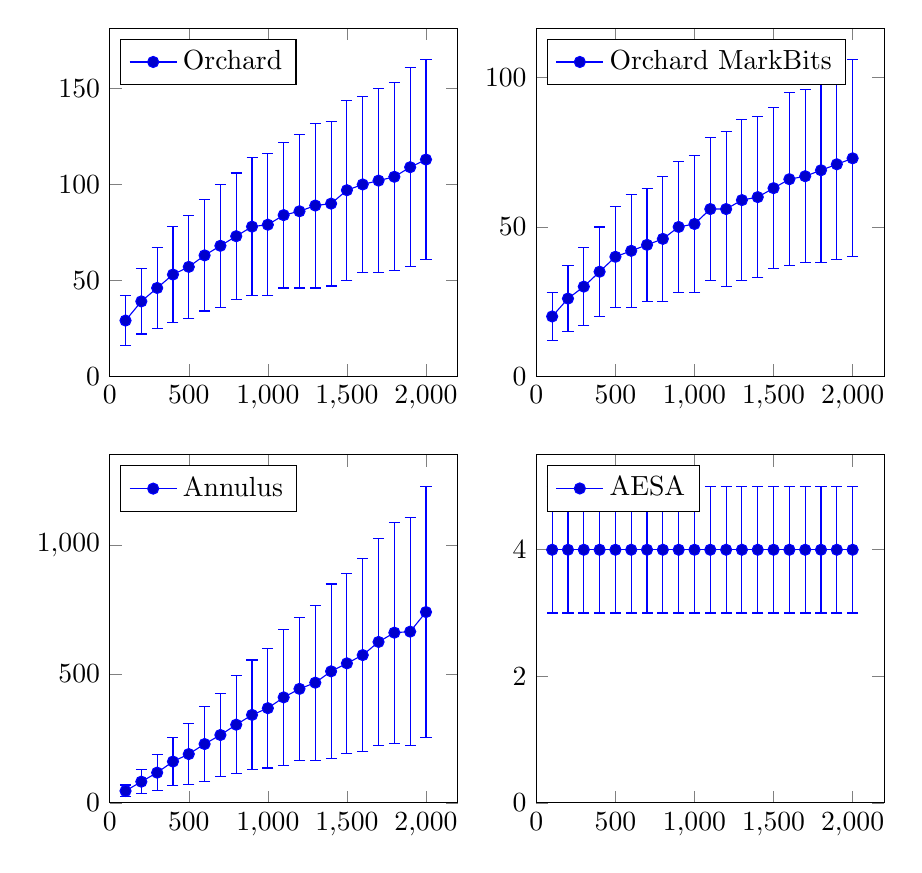
\begin{tikzpicture}
			\begin{groupplot}[group style={group size=2 by 3},height=6cm,width=6cm, legend pos=north west, ymin=0, xmin=0]
				\nextgroupplot
				\addplot+[error bars/.cd, y dir=both,y explicit]
					coordinates {
						(100,29)	+- (13,13)
						(200,39) 	+- (17,17)
						(300,46) 	+- (21,21)
						(400,53) 	+- (25,25)
						(500,57)	+- (27,27)
						(600,63)	+- (29,29)
						(700,68) 	+- (32,32)
						(800,73) 	+- (33,33)
						(900,78) 	+- (36,36)
						(1000,79)	+- (37,37)
						(1100,84)	+- (38,38)
						(1200,86) 	+- (40,40)
						(1300,89) 	+- (43,43)
						(1400,90) 	+- (43,43)
						(1500,97)	+- (47,47)
						(1600,100)	+- (46,46)
						(1700,102) 	+- (48,48)
						(1800,104) 	+- (49,49)
						(1900,109) 	+- (52,52)
						(2000,113)	+- (52,52)
						};
				\addlegendentry{Orchard}
				\nextgroupplot
				\addplot+[error bars/.cd, y dir=both,y explicit]
					coordinates {
						(100,20)	+- (8,8)
						(200,26) 	+- (11,11)
						(300,30) 	+- (13,13)
						(400,35) 	+- (15,15)
						(500,40)	+- (17,17)
						(600,42)	+- (19,19)
						(700,44) 	+- (19,19)
						(800,46) 	+- (21,21)
						(900,50) 	+- (22,22)
						(1000,51)	+- (23,23)
						(1100,56)	+- (24,24)
						(1200,56) 	+- (26,26)
						(1300,59) 	+- (27,27)
						(1400,60) 	+- (27,27)
						(1500,63)	+- (27,27)
						(1600,66)	+- (29,29)
						(1700,67) 	+- (29,29)
						(1800,69) 	+- (31,31)
						(1900,71) 	+- (32,32)
						(2000,73)	+- (33,33)
						};
				\addlegendentry{Orchard MarkBits}
				\nextgroupplot
				\addplot+[error bars/.cd, y dir=both,y explicit]
					coordinates {
						(100,46)	+- (23,23)
						(200,82) 	+- (46,46)
						(300,117) 	+- (69,69)
						(400,160) 	+- (94,94)
						(500,189)	+- (119,119)
						(600,228)	+- (144,144)
						(700,263) 	+- (162,162)
						(800,303) 	+- (190,190)
						(900,341) 	+- (213,213)
						(1000,367)	+- (232,232)
						(1100,409)	+- (264,264)
						(1200,442) 	+- (277,277)
						(1300,466) 	+- (301,301)
						(1400,510) 	+- (339,339)
						(1500,541)	+- (350,350)
						(1600,573)	+- (374,374)
						(1700,624) 	+- (401,401)
						(1800,660) 	+- (429,429)
						(1900,664) 	+- (442,442)
						(2000,740)	+- (487,487)
						};
				\addlegendentry{Annulus}
				\nextgroupplot
				\addplot+[error bars/.cd, y dir=both,y explicit]
					coordinates {
						(100,4)	+- (1,1)
						(200,4) +- (1,1)
						(300,4) +- (1,1)
						(400,4) +- (1,1)
						(500,4)	+- (1,1)
						(600,4)	+- (1,1)
						(700,4)	+- (1,1)
						(800,4) +- (1,1)
						(900,4) +- (1,1)
						(1000,4)	+- (1,1)
						(1100,4)	+- (1,1)
						(1200,4) 	+- (1,1)
						(1300,4) 	+- (1,1)
						(1400,4) 	+- (1,1)
						(1500,4)	+- (1,1)
						(1600,4)	+- (1,1)
						(1700,4) 	+- (1,1)
						(1800,4) 	+- (1,1)
						(1900,4) 	+- (1,1)
						(2000,4)	+- (1,1)
						};
				\addlegendentry{AESA}
			\end{groupplot}
		\end{tikzpicture}
	\end{center}
	\caption{The average amount of distance function calls depending on the size of set $S$ for Orchards Algorithm
		with and without MarkBits, Annulus Method and AESA. The error bars are representing the standard deviation
		of the amount of distance function calls.}
	\label{fig:queryprocessing}
\end{figure}

\section{Conclusions}

\paragraph{Full Search} The results may leave the impression that the Full Search is not a good choice. But this
algorithm remains useful if the set $S$ changes completely with every new query or when $\mathbb{U}$ is no metric space.

\paragraph{Annulus Method} The Annulus Method has a very complex query processing. But on a frequently changing set $S$
a affordable preprocessing. Other algorithms with more complex preprocessing maybe hit its limits on huge sets that
can be handled by the Annulus Method. The Annulus Method was the algorithm with the highest standard deviation during
the benchmarks.

\paragraph{Orchard’s Algorithm with and without marking bits} During query processing the Orchard’s Algorithm with
marking bits consumed on average only 66\% of the distance function calls that the algorithm needed without marking
bits.

\paragraph{AESA} Depending on the benchmarks above, the AESA should be preferred instead of the Orchard’s Algorithm.
Both algorithms have a very complex preprocessing that may not work on very huge sets. But the AESA consumes more less
calls of the distance function. The impact on real world applications should be tested. Beside the Full Search the AESA
was the most stable algorithm.

\section{Future work}

The LAESA\cite{Vidal} algorithm and Metric Trees\cite{Clarkson} are missing in the benchmarks above. These two
algorithms are not parameter free and a optimal implementation for the given domain is not obvious. But both approaches
are promising and their results compared to algorithms of this paper would be interesting.

\begin{thebibliography}{4}
	\bibitem{Clarkson} Clarkson, Kenneth L. "Nearest-neighbor searching and metric space dimensions." Nearest-neighbor
		methods for learning and vision: theory and practice (2006): 15-59.
	\bibitem{Orchard} Orchard, Michael T. "A fast nearest-neighbor search algorithm." Acoustics, Speech, and Signal
		Processing, 1991. ICASSP-91., 1991 International Conference on. IEEE, 1991.
	\bibitem{Ruiz} Ruiz, Enrique Vidal. "An algorithm for finding nearest neighbours in (approximately) constant average
		time." Pattern Recognition Letters 4.3 (1986): 145-157.
	\bibitem{Vidal} Micó, María Luisa, José Oncina, and Enrique Vidal. "A new version of the nearest-neighbour
		approximating and eliminating search algorithm (AESA) with linear preprocessing time and memory requirements."
		Pattern Recognition Letters 15.1 (1994): 9-17.
\end{thebibliography}

\end{document}
